\scanpage{125}
Je vais d'abord passer au deuxième cas de \deleted{\unsure{tels|la}} $Y$ exceptionnels :

Cas où il existe $i_0\in J$ tel que les autom de $(Y,J)$ fixant $i$ forment un groupe d'ordre $3$

\deleted{Ces $Y$ correspondent \unsure{biunivoquement} aux structures la donnée d'un $i_0\in J$ et d'un \unsure{triangulaire} $\unsure{i_0}$ ordre circulaire}

\figure{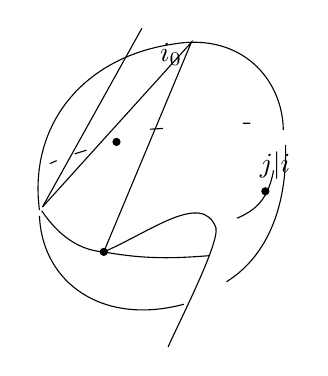
\begin{tikzpicture}[scale=.95]
\draw (0,.9) .. controls (-.15,2.05) and (.6,2.95) .. (1.8,3.12) .. controls (2.7,3.27) and (3.25,2.65) .. (3.26,1.97);
\draw (0,.82) .. controls (.04,-.08) and (.85,-.65) .. (1.93,-.36);
\draw (2.5,-.06) .. controls (3.09,.31) and (3.31,1.02) .. (3.29,1.77);
\draw (.04,.94)--(2.03,3.14)--(.86,.34);
\draw (.04,.94)--(1.37,3.33);
\draw (.03,.89) .. controls (.26,.55) and (.54,.36) .. (.86,.34) .. controls (1.45,.23) and (1.88,.26) .. (2.28,.29);
\draw (.86,.34) .. controls (1.47,.6) and (2.18,1.16) .. (2.36,.66) .. controls (2.4,.44) and (1.88,-.57) .. (1.72,-.93);
\draw (.14,1.52)--(.23,1.56) (.47,1.65)--(.63,1.7) (1.48,1.98)--(1.65,1.99) (2.72,2.06)--(2.82,2.06);
\fill (1.03,1.81) circle (.055);
\fill (.86,.34) circle (.055);
\fill (3.02,1.15) circle (.055);
\draw (2.64,.79) .. controls (2.9,.9) and (3.06,1.05) .. (3.13,1.43);
\node at (1.76,2.98) {$i_0$};
\node at (3.15,1.5) {$\unsure{j|i}$};
\end{tikzpicture}}

(Il revient au $=$ de dire que le groupe autom de $(Y,J)$ est le sous-groupe \inserted{alterné} $\unsure{\mathfrak S|\mathfrak G}_J^+$ de $\unsure{\mathfrak S|\mathfrak G}_J$, ou encore que la configuration est la configuration de la sphère circonscrite au tétraèdre\inserted{\unsure{C. analytique orienté})}. Les $2$ possibilités correspondent aux deux orientations de $J$, soit $\omega_J$ l'une de ces orientations. Le groupe d'isotropie d'un point $i$ est isomorphe au groupe des permutations circulaires sur l'ens des trois autres points qui \unsure{forment|forme} un torseur sous $\inserted{\mu_3=\mu_3(\mathbb C)\simeq}\mathbb Z/3\mathbb Z$, soit $\eta_i$ $(i\in I)$. On a

\figure{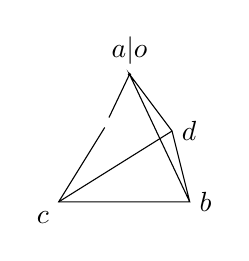
\begin{tikzpicture}[scale=.9]
\coordinate (a) at (1,1.8);
\coordinate (b) at (1.85,0);
\coordinate (c) at (0,0);
\coordinate (d) at (1.6,1.0);
\draw (a)--(.71,1.19);
\draw (.65,1.05)--(c)--(b)--(a)--(d)--(b);
\draw (c)--(d);
\fill (a) circle(.025);
\node[above] at (a) {$\unsure{a|o}$};
\node[right] at (b) {$b$};
\node[below left] at (c) {$c$};
\node[right] at (d) {$d$};
\end{tikzpicture}}

alors
\[
T_i\simeq\mathbb U\mathop{\times}_{\unsure{\deleted{\mathbb Z}|2}\mu_3}\eta_i
\]
où $\mu_3\hookrightarrow\mathbb U$ est l'inclusion canonique.

On

\mspage{124}
